\chapter{System Implementation} \label{s-i}

\section{Introduction} \label{s-i--introduction}

This chapter described the high-level requirements and design of a system that blah blah blah.  The chapter started by describing blah.  The proposed solution was then discussed in section blah followed by blah in section blah, etc.
Blah blah is covered in further detail in Chapter 4 which describes the implementation of blah blah.

From design to implementation a few decisions and technologies changed.

Figure \ref{figure-application-stack-implementation}, shows the revised application stack for the implementation.

\begin{figure}[H]
  \centering
    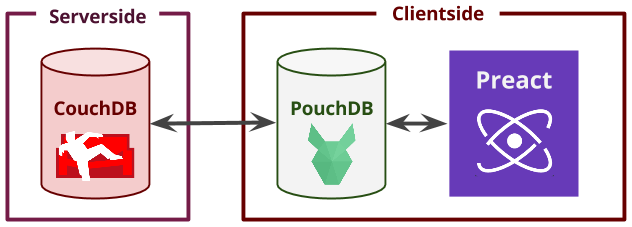
\includegraphics[width=\textwidth,height=\textheight,keepaspectratio]{application_stack_implementation}
  \caption{Overview of how the application stack is structured for the implementation}
  \label{figure-application-stack-implementation}
\end{figure}

The biggest change was the removal of Node.js stack including Express and Passport. As explained fully in section \ref{s-i--data-and-databases} the data manipulation and authentication functionality were handled through CouchDB.

\section{Packages} \label{s-i--packages}

During implementation and research into React and performance another framework was discovered called Preact. Preact, is a framework that attempts to recreate functionality of React but with the focus of performance. Using Preact means a better development experience. \cite{preact} Preact is 3kb in size in comparison to React which is 53kb in size.

The implementation therefor used Preact and was used for rendering views in the artefact.

One principle for software development is DRY (don't repeat yourself). One principle for software development is DRY (don't repeat yourself). ``Every piece of knowledge must have a single, unambiguous, authoritative representation within a system.'' \cite{DRY}

A good example of this is the `moment.js' package used in this artefact, this package handles most date and time related problems. To implement these features is not inherently difficult, but packages such as moment.js offer DRY tried and tested solutions. \cite{moment.js}

\section{Data and Databases} \label{s-i--data-and-databases}

As previously mentioned CouchDB is excellent at master-to-master replication of databases. This means syncing is easily implemented.

\colorbox{pink}{TODO: add diagram here}

The remote database and the local databases sync any changes between themselves, when the local database changes the recipes and brews in state are updated.

In the artefact design data section \ref{a-d--data} and following the decision was to use Node for a Express to handle data coming from the database and Passport to handle user authentication. However through the use of CouchDB and PouchDB it was found that there was no need for either of these technologies.

CouchDB has a user authentication system for handling permission and roles to documents. By default everyone is an admin in what they describe as the `admin party', this is recommended to be disabled but aids development with low barrier to entry when starting a new project.

As the data defines a lot of the structure of the application this authentication system has been leveraged for user authentication for the application.

% \subsection{User Interface}

% push notifications forced the usage of a microservice server due to the GCM
% When registering a user for push notifications there are some best practices in terms of UX.

% Signing up a user with no context is strongly discouraged, the user should always know what they've signed up for through an action. Giving the user even more control by being able to toggle the notifications after initially registering is recommended. \cite{best_practises_push_notifications}

\section{Interesting Problems} \label{s-i--interesting-problems}

During the implementation of this project several issues came up. This section discusses some of these issues.

Using newer technologies such as Webpack, ESLint, Babel and Preact come with difficulties. Due to sometimes the lack of support found online and even some issues can be so new they haven't been documented yet.

For example, with Preact during implmentation there was an issue with a feature from React not being supported. This was short-circuit boolean templating, the author then reported this bug which was then fixed. Here having the Preact project as an Open Source project meant this could be fixed not just for this artefact but future users of Preact.

% describe this better

Handling cache while developing was an issue in the implementation. Initially flushing the cache of the artefact files was done manually however later it was found that the Chrome Developer Tools has options to stop the Service Worker from caching.

\colorbox{pink}{TODO: add dev tools pic here}

Having to depend on the Brauhaus package due to a lack of home-brewing knowledge resulted in having to implement more of the library than potentially needed. This reflects the lack of control of final code expressed in section \ref{l-r--frameworks} discussing frameworks.

\section{Summary} \label{s-i--summary}

This chapter described the implementation of blah blah, which was based on the design described in Chapter 3. The implementation was introduced in section x and blah blah blah. Once the general implementation details had been introduced, several interesting implementation problems were addressed in section q, including the detailed coverage of blah blah.

\section{Testing and Evaluation} \label{s-i--testing-and-evaluation}

\subsection{Introduction} \label{s-i--t-a-e--i}

Chapters 3 and 4 described the design and implementation of blah blah, a system that blah blah blah.  In this chapter, we present a testing method and its results that show blah blah blah.  The chapter is organised as follows:  Section x introduces blah and describes blah.  Next, section y presents blah, etc.
The results of the tests are summarised in section z, before the solution is evaluated in section qqq.
Write what you did, why you did it and how you did it here.

\subsection{Testing Summary} \label{s-i--testing-summary}

In total over n tests were executed. Each test was blah blah blah, and this data was then used to blah. The tests illustrate that blah blah. In the next section, this is evaluated and the extent to which it supports the thesis is discussed.

\colorbox{pink}{TODO: talk about travis}

% travis, tape, jsdom
% use of psi, and webpagetest to evaluate performance budget

\section{Evaluation} \label{s-i--evaluation}

Chapter 1 highlighted the problem of blah blah blah. Chapter 2 reviewed the state-of-the-art in blah and blah.  Chapter 3 identified a set of technical requirements underpinning the development of blah, and the implementation of a blah blah was described in Chapter 4.

The testing described in section x demonstrates that blah blah blah. In this section therefore, we evaluate the implementation and discuss issues in the underlying technologies that the implementation has highlighted.

\subsection{Requirements Review} \label{s-i--requirements-review}

This section reviews the implemented platform, referring back to the requirements to identify the extent to which each has been fulfilled, and reflecting on their relevance for future work. Each of the requirements is reintroduced and discussed in turn.
Refer back to each specified requirement and discuss...


\subsection{Artefact Review} \label{s-i--artefact-review}

This section reviews the implemented platform, referring back to the requirements to identify the extent to which each has been fulfilled, and reflecting on their relevance for future work. Each of the requirements is reintroduced and discussed in turn.
Refer back to each specified requirement and discuss...

\section{Testing and Evaluation Summary} \label{s-i--testing-and-evaluation-summary}

This chapter introduced blah and blah.  In section x a series of tests were described which demonstrated blah blah.
An evaluation of blah blah was then presented in section y.  Section z revisited the requirements described in Chapter 3 and identified that blah blah blah. Finally in section q the aspects of blah blah were discussed.
